The main configuration parameters of the proposed router are summarized as follows:

\begin{itemize}
    \item \textbf{Topology and Node Definition:}

    The design is based on a $3 \times 3$ two-dimensional mesh topology, in which nine processing elements communicate through interconnected routers. Each router is identified by its Cartesian coordinates (x,y), where each coordinate ranges from 0 to 2. This coordinate-based representation provides a direct way to identify the position of each node in the network. 

    \item \textbf{Port Configuration:}

    Each router contains five ports, including one local port connected to the processing element and four directional ports connected to the north, south, west, and east neighboring routers. This five-port organization defines the communication interface of the router in the target mesh network. 
\[
\texttt{port\_t} \in \{\texttt{LOCAL}, \texttt{NORTH}, \texttt{SOUTH}, \texttt{WEST}, \texttt{EAST}\}.
\]
    \item \textbf{Packet and Flit Configuration:}

    For data transmission, packets are divided into 32-bit flits. The supported flit types include head flits, body flits, tail flits, and head-tail flits. Among them, the head flit carries the control and routing information required for packet forwarding. This information is organized into several header fields, including source and destination coordinates, flit type, packet length, virtual-channel information, and message-related fields. The header format and the detailed field definitions are shown in Figure~\ref{fig:header_format} and Table~\ref{tab:header_flit_fields}, respectively.
\[
\texttt{flit\_type\_t} \in \{\texttt{FLIT\_HEAD}, \texttt{FLIT\_BODY}, \texttt{FLIT\_TAIL}, \texttt{FLIT\_HEADTAIL}\}.
\]

\begin{figure}[htbp]
    \centering
    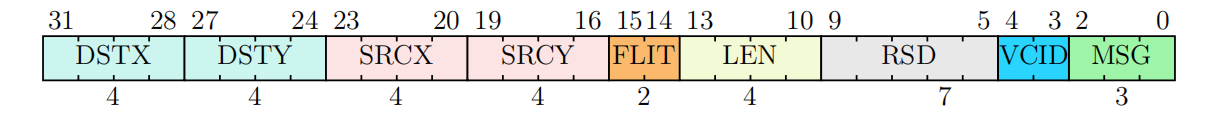
\includegraphics[width=0.8\textwidth]{images/ch3_design_and_implementation/header_flit_field.png}
    \caption{Header flit format and field definitions}
    \label{fig:header_format}
\end{figure}

\begin{table}[htbp]
    \centering
    \caption{Header Flit Fields}
    \label{tab:header_flit_fields}
    \begin{tabular}{llll}
        \hline
        \textbf{Field Name} & \textbf{Bit Slice} & \textbf{Width} & \textbf{Description} \\
        \hline
        DSTX & [31:28] & 4 & Destination ID. \\
        DSTY & [27:24] & 4 & Destination ID. \\
        SRCX & [23:20] & 4 & Source ID. \\
        SRCY & [19:16] & 4 & Source ID. \\
        FLIT & [15:14] & 2 & Flit Type. \\
        LEN  & [13:10] & 4 & Packet Length. \\
        VCID & [4:3]   & 2 & Next Hop IVC ID. \\
        MSG  & [2:0]   & 3 & Message Class. \\
        \hline
    \end{tabular}
\end{table}

    \item \textbf{Virtual Channel Configuration:}

    To support virtual-channel flow control, each router contains five ports, and each port is associated with both input-side and output-side virtual channels. Specifically, each input port contains four input virtual channels (IVCs), and each output port contains four output virtual channels (OVCs). Therefore, one router includes a total of 20 input virtual channels and 20 output virtual channels. These virtual channels provide the buffering and allocation resources required for flit storage, channel assignment, and packet forwarding in the router design.
\end{itemize}
